\documentclass[a4paper,11pt,dvipdfmx]{ujarticle}
% パッケージ
\usepackage{graphicx}
\usepackage{url}
% レイアウト指定を記述したファイルの読み込み
\input{layout}

% タイトルと氏名を変更せよ．
\title{日本におけるデジタル化の状況}
\author{G685112026 米倉 和志}

\begin{document}

\maketitle %ここにタイトルが入る

% ここから本文
% 節見出し: \section{}
% を使う

\section{ブローバンドの整備状況}

% 本文(1)
%  参考文献の参照: \cite{}
%  図番号の参照： \ref{}
% を使う
% 文献データベースのキーワードは oecd と imd
% になっている．
OECDによるブローバンド回線の普及に関する調査\cite{oecd}によると、図\ref{zu1}に示すように、日本における100人あたりの光ファイバー回線の加入者数は29.0で、韓国、スウェーデン、ノルウェーに続いて第４位になっている。

\begin{figure}[htbp]
    \centering
    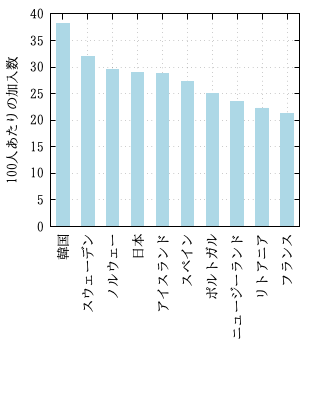
\includegraphics{fig12.png}
    \caption{光ファイバー回線の加入者数(100人あたり)}
    \label{zu1}
\end{figure}
% 図の挿入
% \includegraphics{}
% を
% \begin{figure}[htbp]
% \end{figure}
% で囲み
% \caption{}
% で図のタイトルを入れる．
% \label{}
% を使って図番号が参照できるようにする
% また，
% \centering
% で図が中央に来るようにする

% ーーー
% 節見出し(2)
\section{デジタル競争力ランキング}
% 本文(2)
国際経営開発研究所(IMD)の調査\cite{imd}
によると、日本のデジタル競争力のランキングは表\ref{hyo1}
に示すように、調査対象の64カ国中、総合で28位、技術分野で30位となっている。

\begin{table}[htbp]
    \centering
    \caption{デジタル競争力ランキング(64カ国中)}
    \label{hyo1}
    \begin{tabular}{|c|c|c|} 
        \hline
       国 & 総合 & 技術 \\
       \hline
       米国 & １位 & ４位 \\  
       \hline
       香港 & ２位 & １０位 \\  
       \hline
       スウェーデン & ３位 & ８位 \\  
       \hline
       デンマーク & ４位 & ２位 \\  
       \hline
       シンガポール & ５位 & ３位 \\  
       \hline
       \hline
       韓国 & １２位 & １３位 \\
       \hline
       中国 & １５位 & ２０位 \\  
       \hline
       \hline
       日本 & ２８位 & ３０位 \\ 
       \hline
       \end{tabular} 

\end{table}

% 表の挿入
% \begin{tabular}
% \end{tabular}    
% による表の記述を 
% \begin{table}[htbp]
% \end{table}
% で囲み
% \caption{}
% で表のタイトルを入れる．
% \label{}
% を使って表番号が参照できるようにする
% また，
% \centering
% で表が中央に来るようにする

% ーーー
% 見出し(3)
% 考察
\section{考察}

デジタル競争力ランキング表\ref{hyo1}から以下のことがわかる
\begin{itemize}
    \item 米国の技術分野は４位で総合順位は１位
    \item スウェーデンの技術分野は８位で総合順位は３位
    \item デンマークの技術分野は２位で総合順位は４位
\end{itemize} 
ここから技術分野で高い順位を残した国は、総合ランキングでも高い順位を残す傾向にあることがわかる \\
また日本はアジアの先進国の中でもデジタル競争力ランキングは低い順位である

%
% \begin{itemize}
% \end{itemize}
% を使って箇条書きで記述する

% ここに参考文献が入る
%
\bibliographystyle{junsrt}
\bibliography{exercise.bib}

\end{document}